\documentclass[tikz,border=3pt]{standalone}
\usepackage[utf8]{inputenc}
\usepackage[T1]{fontenc}
\usepackage{lmodern}
\renewcommand{\familydefault}{\sfdefault}
\usepackage{sansmath}\sansmath
\usepackage{chemfig}
\usepackage{pgfplots}\pgfplotsset{compat=1.18,/pgf/number format/use comma,/pgf/number format/1000 sep={.}}
\usetikzlibrary{arrows.meta,calc,positioning,decorations.pathmorphing,patterns}
% paleta del sitio
\definecolor{nar}{HTML}{E8680C}\definecolor{narc}{HTML}{FFB35C}\definecolor{hielo}{HTML}{FFF3E8}
\definecolor{tinta}{HTML}{1D1D1F}\definecolor{gris}{HTML}{6E6E73}\definecolor{lila}{HTML}{7C5CF0}
\definecolor{azul}{HTML}{2F6FD6}\definecolor{menta}{HTML}{17A673}\definecolor{coral}{HTML}{E8342A}
\tikzset{cel/.style={draw=gris,fill=hielo,line width=0.9pt},nuc/.style={draw=gris!70,line width=0.6pt},
fib/.style={gris!55,line width=0.35pt},eti/.style={font=\footnotesize,text=tinta,align=center},
num/.style={circle,draw=nar,fill=white,text=nar,font=\small\bfseries,inner sep=1.2pt,minimum size=13pt},
fl/.style={-{Stealth[length=2.6mm]},gris,line width=0.9pt}}
\begin{document}
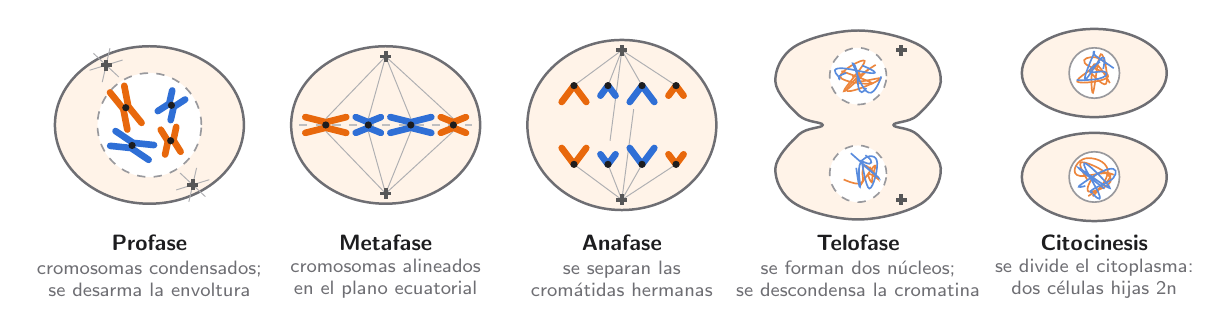
\begin{tikzpicture}[font=\small]
\draw[cel] (0,0) ellipse (1.2 and 1);
\draw[nuc,fill=white,dashed] (0,0) circle (0.66);
\begin{scope}[shift={(-0.3,0.22)},rotate=25]\draw[nar,line width=2.4pt,line cap=round,line join=round] (-0.1,0.26)--(-0.035,0)--(-0.1,-0.26);\end{scope}
\begin{scope}[shift={(-0.3,0.22)},rotate=25]\draw[nar,line width=2.4pt,line cap=round,line join=round] (0.1,0.26)--(0.035,0)--(0.1,-0.26);\end{scope}
\fill[tinta] (-0.3,0.22) circle (1.3pt);
\begin{scope}[shift={(0.28,0.25)},rotate=-35]\draw[azul,line width=2.4pt,line cap=round,line join=round] (-0.1,0.16)--(-0.035,0)--(-0.1,-0.16);\end{scope}
\begin{scope}[shift={(0.28,0.25)},rotate=-35]\draw[azul,line width=2.4pt,line cap=round,line join=round] (0.1,0.16)--(0.035,0)--(0.1,-0.16);\end{scope}
\fill[tinta] (0.28,0.25) circle (1.3pt);
\begin{scope}[shift={(-0.22,-0.26)},rotate=70]\draw[azul,line width=2.4pt,line cap=round,line join=round] (-0.1,0.26)--(-0.035,0)--(-0.1,-0.26);\end{scope}
\begin{scope}[shift={(-0.22,-0.26)},rotate=70]\draw[azul,line width=2.4pt,line cap=round,line join=round] (0.1,0.26)--(0.035,0)--(0.1,-0.26);\end{scope}
\fill[tinta] (-0.22,-0.26) circle (1.3pt);
\begin{scope}[shift={(0.27,-0.2)},rotate=10]\draw[nar,line width=2.4pt,line cap=round,line join=round] (-0.1,0.16)--(-0.035,0)--(-0.1,-0.16);\end{scope}
\begin{scope}[shift={(0.27,-0.2)},rotate=10]\draw[nar,line width=2.4pt,line cap=round,line join=round] (0.1,0.16)--(0.035,0)--(0.1,-0.16);\end{scope}
\fill[tinta] (0.27,-0.2) circle (1.3pt);
\draw[fib] (-0.55,0.76)--(-0.34,0.825);
\draw[fib] (-0.55,0.76)--(-0.501,0.975);
\draw[fib] (-0.55,0.76)--(-0.711,0.91);
\draw[fib] (-0.55,0.76)--(-0.76,0.695);
\draw[fib] (-0.55,0.76)--(-0.599,0.545);
\draw[fib] (-0.55,0.76)--(-0.389,0.61);
\draw[fib] (0.55,-0.76)--(0.76,-0.695);
\draw[fib] (0.55,-0.76)--(0.599,-0.545);
\draw[fib] (0.55,-0.76)--(0.389,-0.61);
\draw[fib] (0.55,-0.76)--(0.34,-0.825);
\draw[fib] (0.55,-0.76)--(0.501,-0.975);
\draw[fib] (0.55,-0.76)--(0.711,-0.91);
\fill[tinta!75] (-0.62,0.735) rectangle (-0.48,0.785);\fill[tinta!75] (-0.575,0.69) rectangle (-0.525,0.83);
\fill[tinta!75] (0.48,-0.785) rectangle (0.62,-0.735);\fill[tinta!75] (0.525,-0.83) rectangle (0.575,-0.69);
\draw[cel] (3,0) ellipse (1.2 and 1);
\draw[gris!45,dashed] (1.9,0)--(4.1,0);
\draw[fib] (3,0.87)--(2.24,0.08);
\draw[fib] (3,-0.87)--(2.24,-0.08);
\draw[fib] (3,0.87)--(2.78,0.08);
\draw[fib] (3,-0.87)--(2.78,-0.08);
\draw[fib] (3,0.87)--(3.32,0.08);
\draw[fib] (3,-0.87)--(3.32,-0.08);
\draw[fib] (3,0.87)--(3.86,0.08);
\draw[fib] (3,-0.87)--(3.86,-0.08);
\begin{scope}[shift={(2.24,0)},rotate=90]\draw[nar,line width=2.4pt,line cap=round,line join=round] (-0.1,0.26)--(-0.035,0)--(-0.1,-0.26);\end{scope}
\begin{scope}[shift={(2.24,0)},rotate=90]\draw[nar,line width=2.4pt,line cap=round,line join=round] (0.1,0.26)--(0.035,0)--(0.1,-0.26);\end{scope}
\fill[tinta] (2.24,0) circle (1.3pt);
\begin{scope}[shift={(2.78,0)},rotate=90]\draw[azul,line width=2.4pt,line cap=round,line join=round] (-0.1,0.16)--(-0.035,0)--(-0.1,-0.16);\end{scope}
\begin{scope}[shift={(2.78,0)},rotate=90]\draw[azul,line width=2.4pt,line cap=round,line join=round] (0.1,0.16)--(0.035,0)--(0.1,-0.16);\end{scope}
\fill[tinta] (2.78,0) circle (1.3pt);
\begin{scope}[shift={(3.32,0)},rotate=90]\draw[azul,line width=2.4pt,line cap=round,line join=round] (-0.1,0.26)--(-0.035,0)--(-0.1,-0.26);\end{scope}
\begin{scope}[shift={(3.32,0)},rotate=90]\draw[azul,line width=2.4pt,line cap=round,line join=round] (0.1,0.26)--(0.035,0)--(0.1,-0.26);\end{scope}
\fill[tinta] (3.32,0) circle (1.3pt);
\begin{scope}[shift={(3.86,0)},rotate=90]\draw[nar,line width=2.4pt,line cap=round,line join=round] (-0.1,0.16)--(-0.035,0)--(-0.1,-0.16);\end{scope}
\begin{scope}[shift={(3.86,0)},rotate=90]\draw[nar,line width=2.4pt,line cap=round,line join=round] (0.1,0.16)--(0.035,0)--(0.1,-0.16);\end{scope}
\fill[tinta] (3.86,0) circle (1.3pt);
\fill[tinta!75] (2.93,0.845) rectangle (3.07,0.895);\fill[tinta!75] (2.975,0.8) rectangle (3.025,0.94);
\fill[tinta!75] (2.93,-0.895) rectangle (3.07,-0.845);\fill[tinta!75] (2.975,-0.94) rectangle (3.025,-0.8);
\draw[cel] (6,0) ellipse (1.2 and 1.08);
\draw[fib] (6,0.95)--(5.392,0.5);
\draw[fib] (6,-0.95)--(5.392,-0.5);
\draw[fib] (6,0.95)--(5.824,0.5);
\draw[fib] (6,-0.95)--(5.824,-0.5);
\draw[fib] (6,0.95)--(6.256,0.5);
\draw[fib] (6,-0.95)--(6.256,-0.5);
\draw[fib] (6,0.95)--(6.688,0.5);
\draw[fib] (6,-0.95)--(6.688,-0.5);
\draw[fib] (6,0.95)--(5.85,-0.2);
\draw[fib] (6,-0.95)--(6.15,0.2);
\begin{scope}[shift={(5.392,0.5)},rotate=0]\draw[nar,line width=2.4pt,line cap=round,line join=round] (-0.156,-0.208)--(0,0)--(0.156,-0.208);\end{scope}
\fill[tinta] (5.392,0.5) circle (1.3pt);
\begin{scope}[shift={(5.392,-0.5)},rotate=180]\draw[nar,line width=2.4pt,line cap=round,line join=round] (-0.156,-0.208)--(0,0)--(0.156,-0.208);\end{scope}
\fill[tinta] (5.392,-0.5) circle (1.3pt);
\begin{scope}[shift={(5.824,0.5)},rotate=0]\draw[azul,line width=2.4pt,line cap=round,line join=round] (-0.096,-0.128)--(0,0)--(0.096,-0.128);\end{scope}
\fill[tinta] (5.824,0.5) circle (1.3pt);
\begin{scope}[shift={(5.824,-0.5)},rotate=180]\draw[azul,line width=2.4pt,line cap=round,line join=round] (-0.096,-0.128)--(0,0)--(0.096,-0.128);\end{scope}
\fill[tinta] (5.824,-0.5) circle (1.3pt);
\begin{scope}[shift={(6.256,0.5)},rotate=0]\draw[azul,line width=2.4pt,line cap=round,line join=round] (-0.156,-0.208)--(0,0)--(0.156,-0.208);\end{scope}
\fill[tinta] (6.256,0.5) circle (1.3pt);
\begin{scope}[shift={(6.256,-0.5)},rotate=180]\draw[azul,line width=2.4pt,line cap=round,line join=round] (-0.156,-0.208)--(0,0)--(0.156,-0.208);\end{scope}
\fill[tinta] (6.256,-0.5) circle (1.3pt);
\begin{scope}[shift={(6.688,0.5)},rotate=0]\draw[nar,line width=2.4pt,line cap=round,line join=round] (-0.096,-0.128)--(0,0)--(0.096,-0.128);\end{scope}
\fill[tinta] (6.688,0.5) circle (1.3pt);
\begin{scope}[shift={(6.688,-0.5)},rotate=180]\draw[nar,line width=2.4pt,line cap=round,line join=round] (-0.096,-0.128)--(0,0)--(0.096,-0.128);\end{scope}
\fill[tinta] (6.688,-0.5) circle (1.3pt);
\fill[tinta!75] (5.93,0.925) rectangle (6.07,0.975);\fill[tinta!75] (5.975,0.88) rectangle (6.025,1.02);
\fill[tinta!75] (5.93,-0.975) rectangle (6.07,-0.925);\fill[tinta!75] (5.975,-1.02) rectangle (6.025,-0.88);
\draw[cel] plot[smooth cycle,tension=0.6] coordinates {(9,1.2) (9.8,1) (10.05,0.55) (9.75,0.12) (9.45,0) (9.75,-0.12) (10.05,-0.55) (9.8,-1) (9,-1.2) (8.2,-1) (7.95,-0.55) (8.25,-0.12) (8.55,0) (8.25,0.12) (7.95,0.55) (8.2,1)};
\draw[nuc,fill=white,dashed] (9,0.62) circle (0.36);
\draw[nar!80,line width=0.6pt] plot[smooth,tension=0.9] coordinates {(8.789,0.685) (9.179,0.528) (8.775,0.609) (9.084,0.813) (8.82,0.429) (9.135,0.71)};
\draw[nar!80,line width=0.6pt] plot[smooth,tension=0.9] coordinates {(9.223,0.763) (8.979,0.564) (9.287,0.588) (8.869,0.43) (9.02,0.65) (8.929,0.607)};
\draw[azul!80,line width=0.6pt] plot[smooth,tension=0.9] coordinates {(9.053,0.755) (9.197,0.658) (8.748,0.719) (8.766,0.592) (8.76,0.62) (8.85,0.661)};
\draw[azul!80,line width=0.6pt] plot[smooth,tension=0.9] coordinates {(9.294,0.616) (9.133,0.411) (8.944,0.749) (8.981,0.696) (9.019,0.435) (9.104,0.47)};
\fill[tinta!75] (9.48,0.925) rectangle (9.62,0.975);\fill[tinta!75] (9.525,0.88) rectangle (9.575,1.02);
\draw[nuc,fill=white,dashed] (9,-0.62) circle (0.36);
\draw[nar!80,line width=0.6pt] plot[smooth,tension=0.9] coordinates {(9.262,-0.691) (9.135,-0.62) (9.171,-0.728) (9.184,-0.643) (9.209,-0.517) (9.027,-0.77)};
\draw[nar!80,line width=0.6pt] plot[smooth,tension=0.9] coordinates {(9.145,-0.532) (9.25,-0.677) (9.108,-0.521) (9.058,-0.577) (9.036,-0.739) (8.817,-0.692)};
\draw[azul!80,line width=0.6pt] plot[smooth,tension=0.9] coordinates {(9.092,-0.385) (9.161,-0.447) (9.142,-0.492) (9.035,-0.471) (9.26,-0.668) (8.908,-0.359)};
\draw[azul!80,line width=0.6pt] plot[smooth,tension=0.9] coordinates {(9.045,-0.441) (9.144,-0.807) (9.237,-0.447) (9.034,-0.474) (9.024,-0.787) (8.977,-0.544)};
\fill[tinta!75] (9.48,-0.975) rectangle (9.62,-0.925);\fill[tinta!75] (9.525,-1.02) rectangle (9.575,-0.88);
\draw[cel] (12,0.66) ellipse (0.92 and 0.56);
\draw[nuc,fill=white] (12,0.66) circle (0.32);
\draw[nar!80,line width=0.6pt] plot[smooth,tension=0.9] coordinates {(12.167,0.766) (12.009,0.861) (11.879,0.786) (12.175,0.614) (11.784,0.551) (12.042,0.753)};
\draw[nar!80,line width=0.6pt] plot[smooth,tension=0.9] coordinates {(12.197,0.532) (12,0.773) (11.983,0.409) (12.083,0.899) (12.149,0.524) (11.926,0.7)};
\draw[azul!80,line width=0.6pt] plot[smooth,tension=0.9] coordinates {(12.247,0.721) (12.016,0.878) (11.99,0.896) (11.884,0.58) (12.1,0.857) (12.113,0.712)};
\draw[azul!80,line width=0.6pt] plot[smooth,tension=0.9] coordinates {(11.777,0.573) (11.896,0.57) (12.102,0.602) (12.134,0.674) (11.94,0.681) (12.071,0.801)};
\draw[cel] (12,-0.66) ellipse (0.92 and 0.56);
\draw[nuc,fill=white] (12,-0.66) circle (0.32);
\draw[nar!80,line width=0.6pt] plot[smooth,tension=0.9] coordinates {(11.915,-0.701) (11.841,-0.473) (12.209,-0.686) (11.928,-0.845) (12.031,-0.622) (12.246,-0.632)};
\draw[nar!80,line width=0.6pt] plot[smooth,tension=0.9] coordinates {(11.923,-0.903) (12.205,-0.632) (11.779,-0.635) (11.891,-0.424) (12.171,-0.573) (11.98,-0.906)};
\draw[azul!80,line width=0.6pt] plot[smooth,tension=0.9] coordinates {(11.982,-0.877) (12.067,-0.899) (11.872,-0.487) (12.197,-0.801) (11.8,-0.545) (12.129,-0.809)};
\draw[azul!80,line width=0.6pt] plot[smooth,tension=0.9] coordinates {(11.886,-0.774) (11.824,-0.761) (12.182,-0.56) (12.243,-0.67) (11.978,-0.82) (11.981,-0.857)};
\node[eti] at (0,-1.5) {\textbf{Profase}};
\node[eti] at (3,-1.5) {\textbf{Metafase}};
\node[eti] at (6,-1.5) {\textbf{Anafase}};
\node[eti] at (9,-1.5) {\textbf{Telofase}};
\node[eti] at (12,-1.5) {\textbf{Citocinesis}};
\node[eti,font=\scriptsize,text=gris] at (0,-1.95) {cromosomas condensados;\\se desarma la envoltura};
\node[eti,font=\scriptsize,text=gris] at (3,-1.95) {cromosomas alineados\\en el plano ecuatorial};
\node[eti,font=\scriptsize,text=gris] at (6,-1.95) {se separan las\\cromátidas hermanas};
\node[eti,font=\scriptsize,text=gris] at (9,-1.95) {se forman dos núcleos;\\se descondensa la cromatina};
\node[eti,font=\scriptsize,text=gris] at (12,-1.95) {se divide el citoplasma:\\dos células hijas 2n};
\end{tikzpicture}
\end{document}
